\subsubsection{Properties}

\begin{description}
		\item[Completness] After KeyGen and Init, for any sequence of calls to
				Update and Refresh producing $x \rightarrow x'$ and $\alpha$,
				then for any query, the proof verifies IFF it returned the
				proper result.
		\item[Security] It is computationally infeasible for an adversary A to
				forge values $q, r, \phi$ which verify, without $F(x, q) = (x,
				r)$.
		\item[Efficiency] Size of authenticator and proof is much smaller than state $x$.
\end{description}

\subsection{Hash tree as ADS}

\begin{itemize}
		\item Hash trees are Merkle trees, using a cryptographic hash function $H$.
		\item Hash value is computed from child nodes: $h \coloneqq(H h_{c_1} || \ldots || h_{c_n})$
		\item Leaf nodes typically contain hashes of (large) data chunks
\end{itemize}

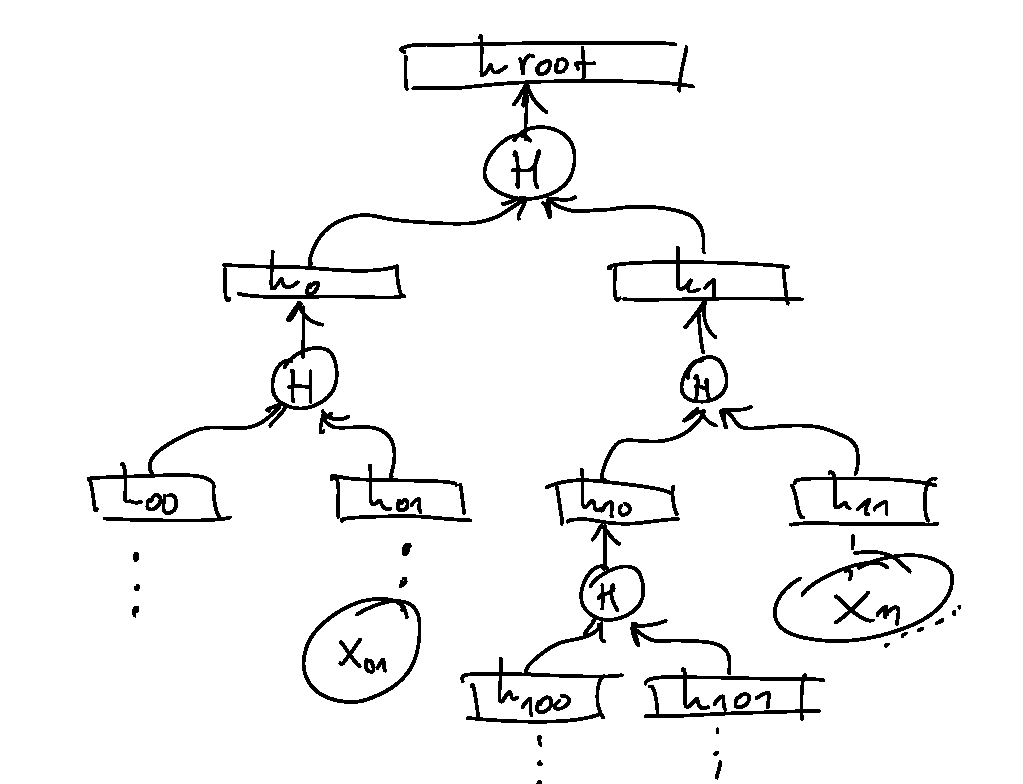
\includegraphics[width=0.6\textwidth]{13_tree}

\subsubsection{Operations}

Assume goal is to authenticate array $X = (x_1, \ldots, x_n)$ of large data
chunks. $F$ has operations $\operatorname{read}(i) \rightarrow x_i$ and
$\operatorname{write}(i, v)$ to read and write elements of $X$.

\paragraph{KeyGen}

Not required

\paragraph{Init}

\begin{itemize}
		\item Compute hash tree on $x_1, \ldots, x_n$
		\item Let $\overline{x}$ consist of $x_1, \ldots, x_n$ plus all
				intermediary nodes of the tree
		\item Let $\alpha$ be the root of the tree
		\item \textbf{Return} $(\overline{x}, \alpha)$
\end{itemize}

\paragraph{Query}

\begin{itemize}
		\item Operation $q$ is $read(i)$
		\item $\phi$ consists of all sibling nodes along the path from leaf $i$
				to root - see picture, marked as red.
		\item \textbf{Return} $(x_i, \phi)$
\end{itemize}

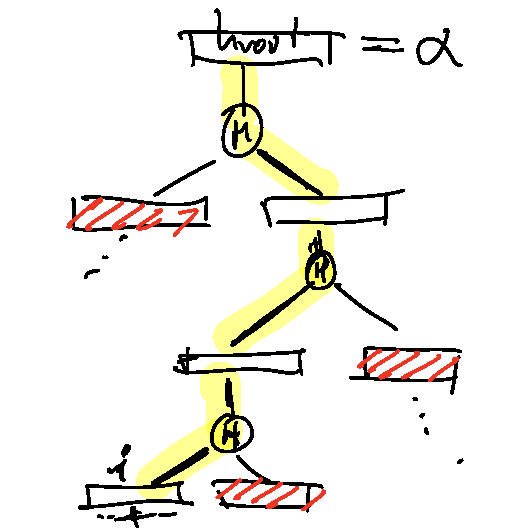
\includegraphics[width=0.5\textwidth]{13_query}

\paragraph{Verify}

\begin{itemize}
		\item Recmopute root hash value $h_q$, starting at $x_i$, using all
				sibling nodes in $\phi$
		\item \textbf{Return} $\alpha = h_q$
\end{itemize}

\paragraph{Update}

\begin{itemize}
		\item Operation $u$ is $\operatorname{write}(i, v)$
		\item $x_i \coloneqq v$
		\item Recompute hash of root node, and nodes in hash tree along path from node $i$ to root
		\item \textbf{Return} $\alpha'$
\end{itemize}

\paragraph{Refresh}

Same as update, by writer.

\subsubsection{Properties}

\begin{description}
		\item[Completness] implicit
		\item[Security] Adversary $A$ breaks security if it can produce $q, r,
				\phi$ which verify, yet $F(x, q) \neq $. This means some
				evluation of $H$ produced a collision, so does not happen
				assuming $H$ is collision-free.
		\item[Efficiency (Space)] $O(n)$ extra storage. In practice using e.g.
				$256-ary$ rather than binary trees helps alleviate the depth.
				Authenticator is small, a few bits. Proof are $O(\log(n) \cdot
				\lambda)$ bits.
		\item[Efficiency (Work)] Update, refresh, query, verify need $O(\log
				n)$, fast.
\end{description}

\subsection{Strong RSA assumption}

Recall ordinary RSA assumption: Given $N, e, x \rgets \mathbb{Z}_N$, it is
infeasible to find $y$ such that $y^e \equiv x \pmod{N}$

Now, strong RSA assumption: Given $N, x \rgets \mathbb{Z}_N$, it is infeasible
to compute $y, z$ such that $y^z \equiv x \pmod{N}$.

That is, the adversary can choose the exponent at will.

\subsection{Accumulator based on RSA}

Let $H : \{0, 1\}^* \rightarrow \mathbb{N}$ be a cryptographic hash function
which outputs distinct primes.

Idea:
\begin{align*}
		\alpha \equiv r^{H(x_1) \cdot \ldots \cdot H(x_n)} \pmod{N}
\end{align*}

Then, $\alpha$ authenticates $x_1, \ldots, x_n$ \textbf{in arbitrary order} for
an initially chosen $r \rgets \mathbb{Z}_N$.

This is a feature. If order is desired, use:
\begin{align*}
		\alpha \equiv r^{H(1 || x_1) \cdot \ldots \cdot H(n || x_n)} \pmod{N}
\end{align*}
